\documentclass[10pt]{article}
\usepackage{icmlko}

\icmlmeta{IP 파운데이션 월드모델}{286}{수 하나}{오늘 만난 벽이 셋인데 전부 같은 수에서 나온다 --- 그리고 그 수를 늘리는 손잡이는 이미 있었다}

\begin{document}

\twocolumn[
\icmlheader

\begin{abstract}
노트 285가 ``다른 새 축들도 전부로 쟀나''를 남겼다. 봤다. \textbf{노트 276의
팝업 후보 검사가 75행 전부로 잰 것이고 그중 59행(79\%)이 유보다.} 학습만으로
다시 재면 \texttt{기간\_주말몫} 이 $+$0.380 $\to$ \textbf{$+$0.187}($n{=}14$),
\texttt{경쟁\_1km} 이 $+$0.319 $\to$ $+$0.292($n{=}14$)다. 오늘 세 번째
엿보기인데 이번 것은 원인이 구조적이다 --- \textbf{팝업의 배포 학습행이
16(관측 14)이라 노트 239의 채택 검사를 \emph{할 수가} 없다.} 도메인마다
무엇이 가능한지 세었다: 검사 ①③(학습 상관, $\ge$30행)과 ②(시간 다섯 조각,
조각마다 60행이니 $\ge$300)를 기준으로 \textbf{열한 중 여섯만 셋 다 되고, 넷은
①③만 되고, 팝업 하나는 아무것도 못 한다.} 그리고 여기서 오늘 하루가 하나로
모인다 --- \textbf{노트 274}(판이 팝업의 개선을 못 본다 · 몫 2.3\% · 문턱
0.435) · \textbf{노트 276 · 281}(챔피언이 팝업의 전용 축을 못 듣는다 ·
16 $<$ 22) · \textbf{이 노트}(팝업에서는 축 채택 검사를 못 한다 · 16 $<$ 30).
\textbf{세 벽이 전부 팝업 학습 16행 하나에서 나온다.} 마지막으로 좋은 소식:
\textbf{그 수를 늘리는 손잡이가 이미 있다.} 노트 133의 넓힌 판(\texttt{wide})이
팝업 학습을 \textbf{16 $\to$ 73}, 유보를 59 $\to$ 116 으로 늘려 검사 ①과
청력 문턱을 \emph{둘 다} 넘긴다. 다만 라벨이 \texttt{organizer\_claim} 이라
\textbf{과제가 바뀐다} --- 노트 283 · 284가 시장 층에서 만난 것과 같은 자리다.
\end{abstract}
]

\section{세 번째 엿보기, 그런데 구조적이다}

노트 285가 자기 채택 근거에서 엿보기를 찾았다(\texttt{category} 의
$H{=}29.4$ 가 유보 포함이었고 학습만은 14.5). 그 노트가 ``다른 새 축들도
전부로 쟀나''를 남겨서 봤다.

\textbf{노트 276이 팝업 후보 열여섯을 거를 때 75행 전부를 썼다.}

\begin{center}\small
\begin{tabular}{lrrr}
\hline
& 전부 & 학습만 & 유보만 \\
\hline
\texttt{기간\_주말몫} & $+$0.380 & \textbf{$+$0.187} & $+$0.458 \\
& ($n{=}66$) & ($n{=}14$) & ($n{=}52$) \\
\texttt{경쟁\_1km} & $+$0.319 & $+$0.292 & $+$0.314 \\
& ($n{=}68$) & ($n{=}14$) & ($n{=}54$) \\
\hline
\end{tabular}
\end{center}

\textbf{79\% 가 유보였다.} 그리고 학습만 쓰면 $n{=}14$ 다 --- 추정이 서는
크기가 아니다.

\paragraph{이건 실수가 아니라 불가능이다} 노트 239가 세운 규약은 ``채택 근거는
학습 구간이다''인데, \textbf{팝업의 학습이 16행이라 그 규약을 지킬 방법이
없다.} 지키면 $n{=}14$ 로 아무것도 못 재고, 안 지키면 엿보기다.

\section{어느 도메인이 검사를 지탱하나}

\begin{figure*}[t]
\centering
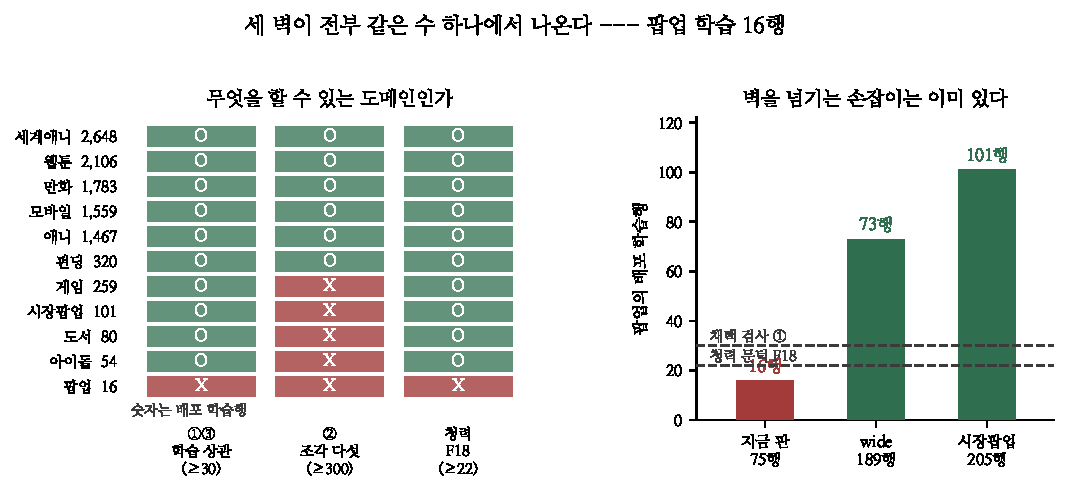
\includegraphics[width=\textwidth]{figs/one.pdf}
\caption{왼쪽 --- 도메인마다 어떤 검사가 가능한가. 오른쪽 --- 팝업의 세 층과
두 문턱.}
\end{figure*}

노트 239 · 256의 검사 셋이 요구하는 행 수를 적어 봤다. 검사 ①③(연도 통제
학습 상관 · 기존 축과 겹침)은 학습 행에서 상관을 재니 최소 30쯤은 있어야
하고, 검사 ②(시간 다섯 조각 부호 일치)는 조각마다 60이 필요하다 --- 노트 257이
\textbf{60 미만에서 검사가 ``전부 탈락''이라는 깨끗한 거짓말}을 하는 것을 봤다.

\begin{center}\small
\begin{tabular}{lrccc}
\hline
도메인 & 학습행 & ①③ & ② & 청력 \\
\hline
세계애니 · 웹툰 & 2,648 · 2,106 & O & O & O \\
만화 · 모바일 · 애니 & 1,783$\sim$1,467 & O & O & O \\
펀딩 & 320 & O & O & O \\
\hline
게임 & 259 & O & \textbf{X} & O \\
시장팝업 & 101 & O & \textbf{X} & O \\
도서 · 아이돌 & 80 · 54 & O & \textbf{X} & O \\
\hline
\textbf{팝업} & \textbf{16} & \textbf{X} & \textbf{X} & \textbf{X} \\
\hline
\end{tabular}
\end{center}

\textbf{열한 중 여섯만 셋 다 되고, 팝업 하나는 아무것도 못 한다.}

\section{세 벽이 같은 수에서 나온다}

여기서 오늘 하루가 하나로 모인다.

\begin{center}\small
\begin{tabular}{llr}
\hline
노트 & 벽 & 팝업의 수 \\
\hline
274 & 판이 개선을 못 본다 & 몫 2.3\%, 문턱 $\Delta\rho{=}0.435$ \\
276 · 281 & 챔피언이 전용 축을 못 듣는다 & 학습 \textbf{16} $<$ 22 \\
\textbf{286} & 축 채택 검사를 못 한다 & 학습 \textbf{16} $<$ 30 \\
\hline
\end{tabular}
\end{center}

앞의 것은 유보 59행에서, 뒤의 둘은 학습 16행에서 온다. 그리고 그 둘은 같은
75행을 시간으로 자른 것이다. \textbf{벽이 셋으로 보였는데 수는 하나였다.}

이것이 노트 276$\sim$282의 일곱 노트가 팝업에서 아무것도 못 얻은 이유다 ---
축이 나빠서가 아니라 \textbf{그 도메인에서는 축을 고를 수도, 배울 수도, 잰
것을 판에 실을 수도 없었다.} 세 번 다른 얼굴로 만났을 뿐이다.

\section{손잡이는 이미 있었다}

\begin{center}\small
\begin{tabular}{lrrl}
\hline
층 & 학습 & 유보 & \\
\hline
지금 판 & 16 & 59 & 셋 다 못 넘음 \\
\textbf{\texttt{wide}}(노트 133) & \textbf{73} & \textbf{116} & 검사 ① · 청력 넘음 \\
시장팝업(노트 284) & 101 & 104 & 검사 ① · 청력 넘음 \\
\hline
\end{tabular}
\end{center}

\textbf{노트 133이 이미 만들어 둔 넓힌 판이 팝업 학습을 73행으로 늘린다.}
검사 ①(30)과 청력 문턱(22)을 둘 다 넘긴다. 검사 ②(300)는 여전히 못 넘는다.
유보도 59 $\to$ 116 이라 검출 문턱이 0.083 에서 0.06 언저리로 내려간다.

\paragraph{그런데 과제가 바뀐다} 넓힌 판은 계수 필터를 풀어
\texttt{organizer\_claim} 라벨을 쓴다. \textbf{노트 283 · 284가 시장 층에서
만난 것과 같은 자리다} --- 라벨 모집단이 달라지므로 판 수를 옛것과 견주면
안 되고, 노트 127이 잰 대로 축을 자동 태깅으로 채우면 팝업이 $+$0.4562 에서
$+$0.1150 으로 무너진다(그래서 넓힌 판은 축을 안 채운다).

\textbf{그러니 이건 ``켜면 되는 손잡이''가 아니라 ``다른 과제로 옮기는
결정''이다.} 노트 224의 규약이 여기 걸린다 --- 과제를 바꾸는 결정은 점수로
정하지 않는다.

\paragraph{남은 것}
\begin{center}\small
\begin{tabular}{ll}
\hline
갈래 & 왜 \\
\hline
넓힌 판에서 다시 & 벽 둘을 넘긴 뒤 노트 276 을 재현해 볼 것 \\
검사 ② 를 못 하는 넷 & 게임 · 시장팝업 · 도서 · 아이돌 \\
노트 276 재검사 & 학습만으로는 $n{=}14$ --- 결론이 서나 \\
과제 결정 & 넓힌 판으로 갈지는 점수 밖에서 \\
\hline
\end{tabular}
\end{center}

\paragraph{규약} \textbf{검사를 걸기 전에 그 도메인이 검사를 지탱하는지
먼저 센다.} 노트 239가 검사 셋을 세울 때 웹툰(2,106행)을 보고 세웠고, 그
검사를 16행짜리 도메인에 그대로 걸었다 --- 지킬 수 없는 규약은 조용히
엿보기가 된다. 그리고 \textbf{벽을 여러 개 만나면 수를 세어 본다} --- 오늘
세 노트가 서로 다른 이야기인 줄 알았는데 같은 16이었다.

\end{document}
